\section{Layered Architecture}

\begin{frame}{Layered Architecture}
    \begin{itemize}
        \item Bisher: Isolierter Microservice pro Funktionalität
        \item Problem: Redundanz in Schnittstellen-Logik (Logging, Authentifizierung, \ldots)
        \item Jetzt: Aufteilung System in Schichten
        \item Ziel: Separation of Concerns \& Layers of isolation \cite{architecturePatterns}
    \end{itemize}
\end{frame}

\begin{frame}{Layered Microservice Architecture: Beispiel E-Commerce}
    \begin{figure}[!h]
        \centering
        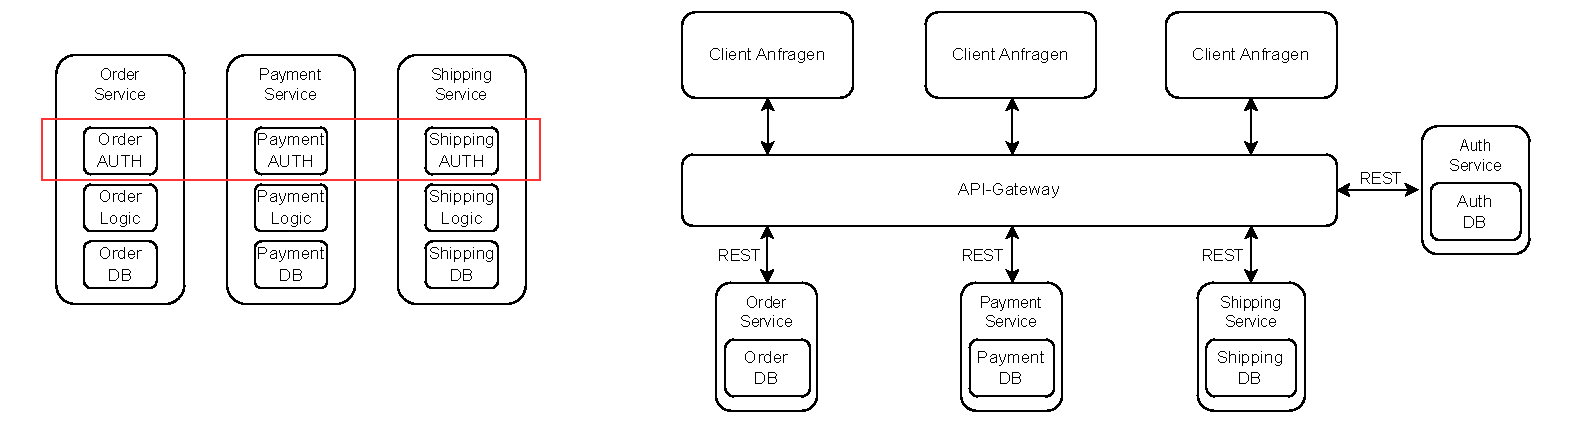
\includegraphics[scale=0.55]{imglib/layered/ecommerce-example}
        \caption{E-Commerce Beispiel mit geschichteter Microservice Architektur}
        \label{fig:layered}
    \end{figure}
\end{frame}

\begin{frame}{Layered Architecture: Agilität}
    \begin{itemize}
        \item Separation of Concerns $\Rightarrow$ kleine autonome Teams
        \item Layers of isolation $\Rightarrow$ hohe Flexibilität
        \item Funktionalitäten wiederverwendbar $\Rightarrow$ Auslieferung in kurzen Intervallen
        \item Kombination mit anderen EA-Mustern sehr sinnvoll
    \end{itemize}
\end{frame}
